\documentclass{bmstu}

\usepackage{pdfpages}

\addbibresource{inc/biblio/sources.bib}

\begin{document}

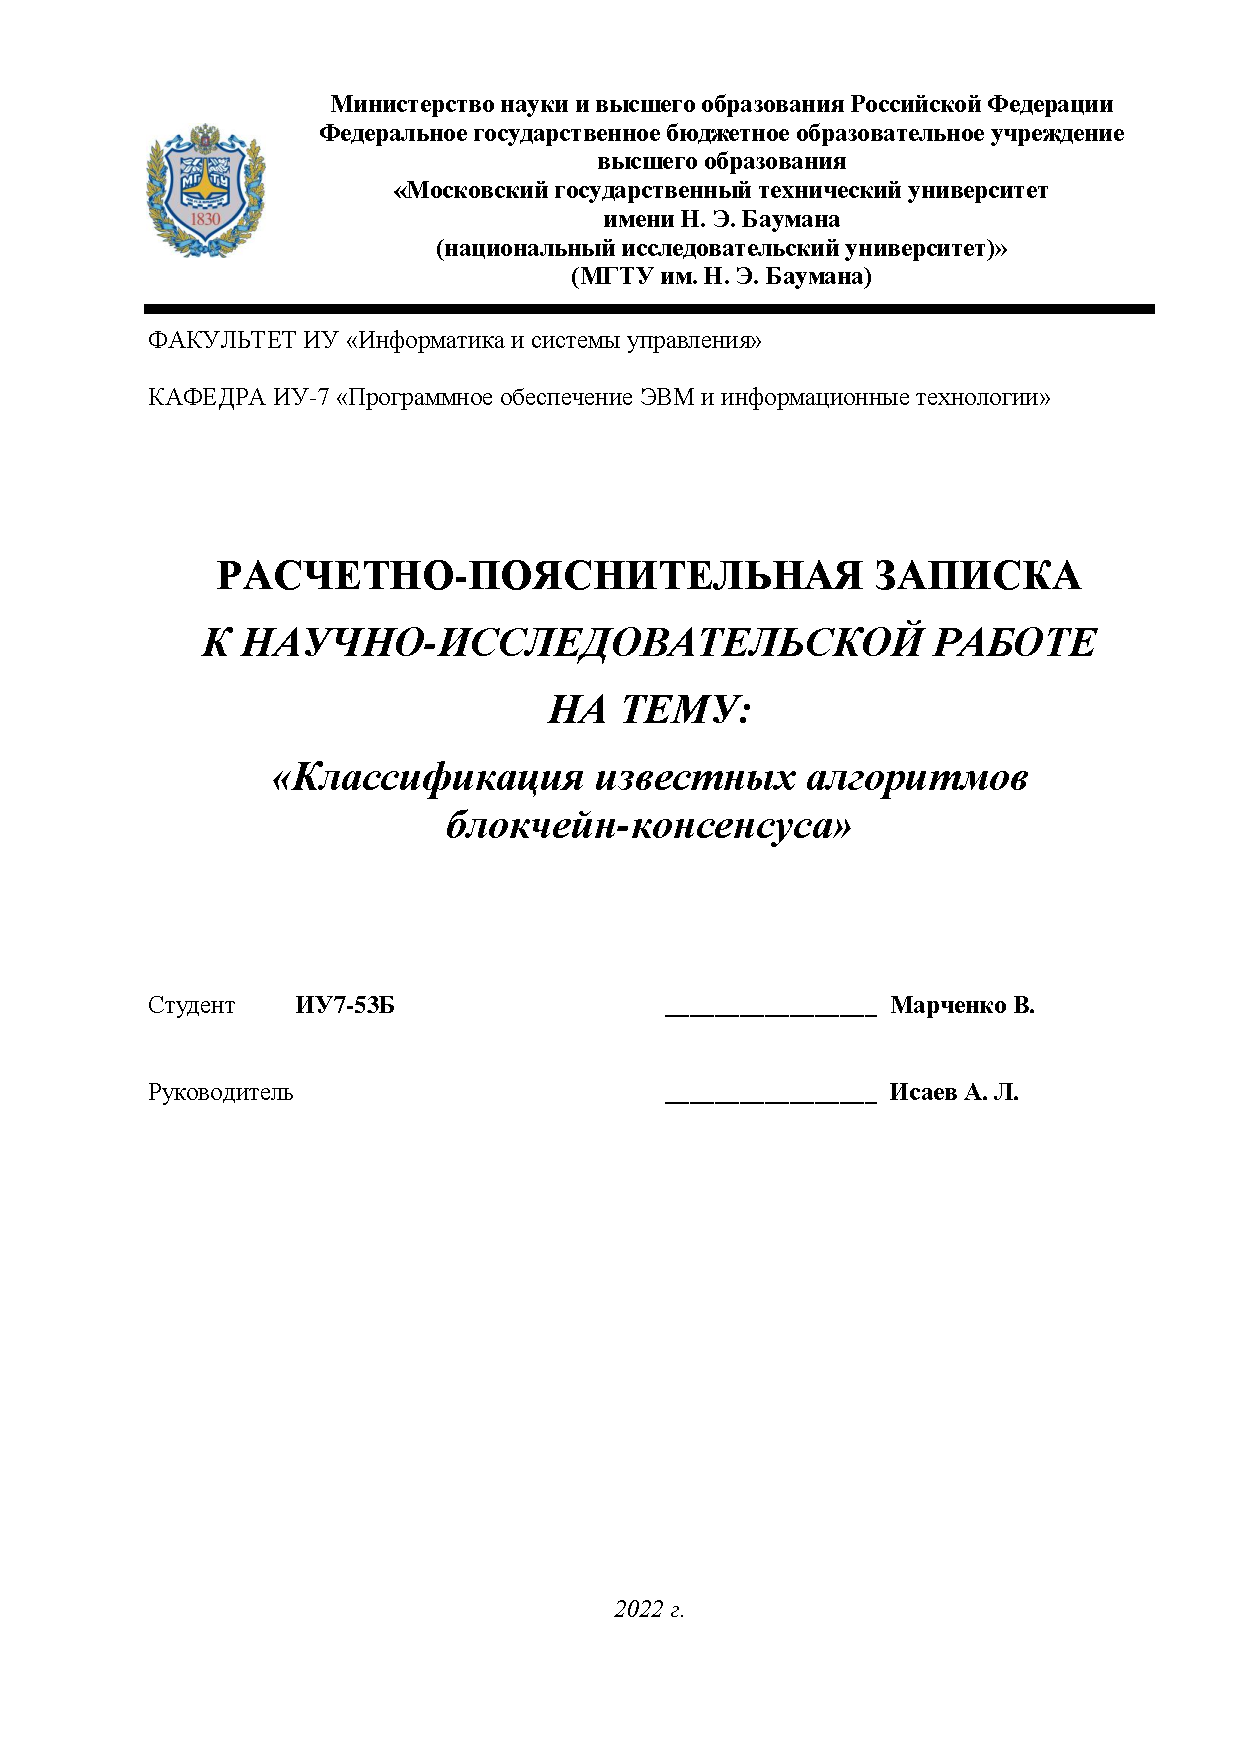
\includepdf[pages=-]{inc/img/title.pdf}

{\centering \chapter*{РЕФЕРАТ}}

Отчет 21 с., 4 рис., 3 табл., 11 источн., 1 прил.

\noindent БЛОКЧЕЙН, КОНСЕНСУС, АЛГОРИТМЫ КОНСЕНСУСА, PROOF OF WORK, PROOF OF STAKE, PROOF OF IMPORTANCE, PROOF OF CAPACITY, HYBRID CONSENSUS

Объектом исследования является технология блокчейн.

Цель работы: классификация существующих алгоритмов блокчейн-консенсуса.

В результате исследования было проведено сравнение пяти алгоритмов блокчейн-консенсуса по трем критериям.

Область применения результатов --- выбор алгоритма консенсуса при создании блокчейна.

Результат работы. 
Выбор механизма консенсуса зависит от целей, которые преследует разработчик при создании блокчейна. 
Меньше всего времени на создание нового блока в сети тратит алгоритм Proof of Stake, наиболее стойкими к двойному расходованию являются механизмы Proof of Work, Hybrid Consensus и Proof of Importance, а наибольшее количество транзакций в секунду позволяет проводить Proof of Importance.

\maketableofcontents

{\centering \chapter*{ПЕРЕЧЕНЬ СОКРАЩЕНИЙ И ОБОЗНАЧЕНИЙ}}

В настоящем отчете о НИР применяют следующие сокращения и обозначения:

\begin{table}[H]
\begin{tabular}{p{3cm}p{13.5cm}}
HC & Алгоритм блокчейн-консенсуса Hybrid Consensus
\tabularnewline
NEM & Криптовалюта New Economy Movement
\tabularnewline
PoC & Алгоритм блокчейн-консенсуса Proof of Capacity
\tabularnewline
PoI & Алгоритм блокчейн-консенсуса Proof of Importance
\tabularnewline
PoS & Алгоритм блокчейн-консенсуса Proof of Stake
\tabularnewline
PoW & Алгоритм блокчейн-консенсуса Proof of Work
\tabularnewline
\end{tabular}
\end{table}

{\centering \chapter*{ВВЕДЕНИЕ}}
\addcontentsline{toc}{chapter}{ВВЕДЕНИЕ}

Блокчейн --- это очередная волна перемен, которая уже начала менять структуру
деловых, социальных и политических связей, а также способы перемещения
средств. 
С другой стороны, блокчейн --- это не просто перемены, а некая сущность, которая никогда не стоит на месте. 
Более 40 ведущих финансовых учреждений и множество фирм в различных отраслях начали осваивать блокчейн --- чтобы снизить транзакционные издержки, ускорить прохождение транзакций, снизить риск мошенничества и устранить посредников. 
Некоторые фирмы пытаются с его помощью перестроить устаревшие системы и сервисы, чтобы вывести их на следующий уровень, а также предложить новые виды услуг \cite[19]{Singhal2019}.

Блокчейн --- это структура данных, которая представляет собой упорядоченный связный список блоков транзакций. 
Каждый блок в цепочке ссылается на предыдущий. 
Блокчейн часто визуализируют как стек с блоками, наложенными друг на друга. 
Первый блок в цепи является основанием стека, т. е. его нижним элементом. 
Визуализация блоков, наложенных друг на друга, приводит к использованию такого термина, как <<высота>> для обозначения расстояния от первого блока до текущего. Последний добавленный в цепь блок является вершиной стека \cite[163]{Antonopoulos2010}.

Блокчейн --- это система записей о переносе любой ценности (а не только денег) по принципу <<от равного к равному>>. 
Это означает, что нет необходимости в посредниках, таких как банки, брокеры или другие службы депонирования, которые служат доверенной третьей стороной \cite[21]{Singhal2019}.

Но как всем в сети договориться о единой универсальной <<истине>> о том, кому что принадлежит, не доверяя никому? 
Все традиционные платежные системы зависят от модели доверия, в которой есть центральный объект, предоставляющий услуги расчетной палаты, в основном проверяющий и выполняющий все транзакции. 
Главное изобретение Сатоши Накамото --- децентрализованный механизм эмерджентного консенсуса. 
Эмерджентный, потому что консенсус не достигается явным образом --- нет выбора или фиксированного момента, когда достигается консенсус. 
Напротив, консенсус --- это возникающий артефакт асинхронного взаимодействия тысяч независимых узлов, следующих простым правилам \cite[181]{Antonopoulos2010}.

Существует множество различных алгоритмов блокчейн-консенсуса. 
Они зависят от блокчейн-сетей и их применения. 
Несмотря на то, что эти алгоритмы различаются по энергопотреблению, безопасности и масштабируемости, все они преследуют одну цель --- обеспечить достоверность всех записей.

Цель научно-исследовательской работы: провести обзор существующих алгоритмов консенсуса для блокчейна и классифицировать их по сформулированным критериям.

Задачи научно-исследовательской работы:

\begin{enumerate}
\item[1)]
исследовать технологию блокчейн;
\item[2)]
исследовать основные механизмы, которые используются в рамках этой технологии;
\item[3)]
проанализировать известные алгоритмы блокчейн-консенсуса;
\item[4)]
сформулировать критерии для сравнения алгоритмов блокчейн-консенсуса;
\item[5)]
сравнить алгоритмы блокчейн-консенсуса по сформулированным критериям.
\end{enumerate}

\chapter{Анализ предметной области}

\section{Технология блокчейн}

Как было сказано ранее, блокчейн --- это структура данных, которая представляет собой упорядоченный связный список блоков транзакций. 
Каждый блок в цепи идентифицируется хэшем, сгенерированным с помощью криптографического алгоритма SHA-256 в заголовке блока. 
Каждый блок ссылается на предыдущий, т. н. родительский блок, через поле <<хэш предыдущего блока>> в заголовке. 
Другими словами, каждый блок содержит хэш своего родителя внутри своего собственного заголовка. 
Последовательность хэшей, связывающих каждый блок с его родителем, создает цепочку, восходящую к первому когда-либо созданному блоку, известному как блок генезиса \cite[163]{Antonopoulos2010}.

Хотя у блока есть только один родитель, он может временно иметь несколько дочерних элементов. 
Каждый из потомков ссылается на тот же блок, что и его родитель, и содержит тот же (родительский) хэш в поле <<хэш предыдущего блока>>. 
Множественные дочерние блоки возникают во время т. н. <<форка>> блокчейна --- временной ситуации, когда разные блоки создаются почти одновременно разными майнерами. 
На рисунке~\ref{img:fork} изображен процесс <<форка>>.

\includeimage
    {fork}
    {f}
    {H}
    {.9\textwidth}
    {Процесс <<форка>> \cite{Sheikh2018}}

\pagebreak
В конце концов, только один дочерний блок становится частью блокчейна, и <<форк>> разрешается. 
Несмотря на то, что блок может иметь более одного дочернего элемента, каждый блок может иметь только одного родителя. 
Это связано с тем, что блок имеет единственное поле <<хэш предыдущего блока>>, ссылающееся на его единственного предка \cite[163]{Antonopoulos2010}.

Поле <<хэш предыдущего блока>> находится внутри заголовка блока и тем самым влияет на хэш текущего блока. 
Дочерний блок изменяется, если меняется родительский. 
Когда родитель каким-либо образом изменяется, его хэш также изменяется. 
Измененный хэш родителя требует изменения поля <<хэш предыдущего блока>> дочернего блока. 
Это, в свою очередь, приводит к изменению хэша потомка, что требует изменения указателя внучатого элемента, который, в свою очередь, изменяет внука и так далее по цепи. 
Данный каскадный эффект гарантирует, что после того, как за блоком последовало некоторое количество поколений, его нельзя изменить без принудительного пересчета всех последующих блоков. 
Поскольку такой пересчет потребовал бы огромных вычислений, существование длинной цепи блоков делает длинную историю блокчейна неизменной, что является ключевой особенностью безопасности криптовалют \cite[164]{Antonopoulos2010}.

В блокчейне самые последние несколько блоков могут быть пересмотрены, если происходит пересчет цепи из-за <<форка>>. 
Но как только происходит углубление в блокчейн за пределы шести блоков, вероятность того, что блоки изменятся, будет уменьшаться. 
Несколько тысяч созданных в цепи блоков --- и цепь --- это устоявшаяся история. Она никогда не изменится \cite[164]{Antonopoulos2010}. 
На рисунке~\ref{img:blockchain} изображена общая структура блокчейна.

\includeimage
    {blockchain}
    {f}
    {H}
    {.7\textwidth}
    {Общая структура блокчейна \cite{Ribera2018}}

\section{Транзакции}

Транзакция в информатике --- неделимая последовательность операций, которая представляет собой логическую единицу работы с данными. 
Транзакции обладают следующими свойствами:

\begin{enumerate}
\item[1)]
атомарность;
\item[2)]
согласованность;
\item[3)]
изоляция;
\item[4)]
устойчивость.
\end{enumerate}

В блокчейне транзакции --- это структуры данных, которые кодируют передачу информации между участниками блокчейн-сети. 
Каждая транзакция является общедоступной записью в публичном реестре \cite[111]{Antonopoulos2010}.

\section{Майнинг}

Майнинг --- это процесс многократного хэширования заголовка блока с изменением одного параметра до тех пор, пока полученный хэш не будет удовлетворять определенным требованиям. 
Результат хэш-функции нельзя определить заранее, и нельзя создать шаблон, который будет создавать определенное значение хэш-функции. 
Эта особенность хэш-функций означает, что единственный способ получить результат хэширования, соответствующий конкретной цели --- это постоянно изменять случайным образом входные данные до тех пор, пока не появится желаемый результат хэширования \cite[192]{Antonopoulos2010}.

\section{Структура блока}

Блок --- это контейнерная структура данных, которая агрегирует транзакции для включения их в публичный реестр. Блок состоит из заголовка, содержащего метаданные, за которым следует длинный список транзакций, составляющих основную часть размера блока. Заголовок блока занимает 80 байт, тогда как средний размер транзакции составляет не менее 250 байт, а в среднем блок содержит более 500 транзакций. Таким образом, полный блок со всеми транзакциями весит в 1000 раз больше заголовка блока \cite[164]{Antonopoulos2010}.

В таблице~\ref{tabular:blockstructure} описана структура блока --- указаны размеры полей в байтах, их названия и описания.

\begin{table}[H]
\caption{Структура блока}
\label{tabular:blockstructure}
\begin{tabular}{|p{3.5cm}|p{4.5cm}|p{7cm}|}
\hline
\textbf{Размер} & \textbf{Поле} & \textbf{Описание}
\tabularnewline
\hline
4 байта & Размер блока & Размер блока в байтах
\tabularnewline
\hline
80 байт & Заголовок блока & Несколько полей, формирующих заголовок блока
\tabularnewline
\hline
1--9 байт & Счетчик транзакций & Количество проведенных транзакций
\tabularnewline
\hline
Переменный & Транзакции & Транзакции, записанные в этом блоке
\tabularnewline
\hline
\end{tabular}
\end{table}

\section{Заголовок блока}

Заголовок блока состоит из трех наборов метаданных блока. Во-первых, это ссылка на хэш предыдущего блока, которая связывает текущий блок в цепи с предыдущим. Второй набор метаданных, а именно сложность, отметка времени и одноразовый номер, относятся к майнингу. Третьей частью метаданных является корень дерева Меркла --- структуры данных, которая используется для эффективного суммирования всех транзакций в блоке \cite[165]{Antonopoulos2010}.

В таблице~\ref{tabular:headerstructure} описана структура заголовка блока --- указаны размеры полей в байтах, их названия и описания.

\begin{table}[H]
\caption{Структура заголовка блока}
\label{tabular:headerstructure}
\begin{tabular}{|p{3.5cm}|p{4.5cm}|p{7cm}|}
\hline
\textbf{Размер} & \textbf{Поле} & \textbf{Описание}
\tabularnewline
\hline
4 байта & Версия & Номер версии для отслеживания обновлений программного обеспечения/протокола
\tabularnewline
\hline
32 байта & Хэш предыдущего блока & Ссылка на хэш предыдущего (родительского) блока в цепи
\tabularnewline
\hline
32 байта & Корень дерева Меркла & Хэш корня дерева Меркла транзакций этого блока
\tabularnewline
\hline
4 байта & Отметка времени & Примерное время создания этого блока в секундах (Unix-время)
\tabularnewline
\hline
4 байта & Сложность & Сложность алгоритма Proof of Work для этого блока
\tabularnewline
\hline
4 байта & Одноразовый номер & Счетчик, используемый для алгоритма Proof of Work
\tabularnewline
\hline
\end{tabular}
\end{table}

\section{Блокчейн-консенсус}

В распределенной системе соглашение является фундаментальной проблемой, и это обычно иллюстрируется задачей византийских генералов \cite{Lamport1982}. 
Блокчейн, являясь распределенной системой, основан на алгоритме консенсуса, который обеспечивает согласование состояний определенных данных между распределенными узлами. 
Алгоритм консенсуса --- это основной компонент, который напрямую определяет поведение такой системы и производительность, которую она может достичь. 
Широкий спектр криптовалют, предназначенных для различных областей применения, определил множество уникальных требований, которые могут быть удовлетворены только с помощью соответствующих механизмов консенсуса. 
Этот факт вызвал потребность не только в изучении применимости существующих алгоритмов консенсуса в новых условиях, но и в разработке новых алгоритмов консенсуса. 
В результате появилось несколько алгоритмов консенсуса, каждый из которых обладает интересными свойствами и уникальными возможностями \cite{Sadek2020}.

\chapter{Классификация алгоритмов блокчейн-консенсуса}

\section{Алгоритмы блокчейн-консенсуса}

\subsection{Алгоритм Proof of Work}

Proof of Work --- это форма криптографического доказательства, в котором одна сторона (доказывающая) доказывает другим (верификаторам), что было затрачено определенное количество конкретных вычислительных усилий \cite{Lachtar2020}.

Этот механизм первоначально был предложен в 1993 году для борьбы с нежелательными электронными письмами и для контроля доступа к общим ресурсам \cite{Dwork1982}.

Благодаря системе <<Биткоин>> алгоритм консенсуса PoW является наиболее известным способом подтверждения транзакций. 
Основная идея состоит в том, чтобы узлы блокчейна, подтверждающие транзакции, проделывали достаточно сложную вычислительную работу --- просчет алгоритма --- результат работы которого был бы легко и быстро проверяем другими узлами сети.

Первый узел, который полностью провел все необходимые вычисления, получает вознаграждение от блокчейна. 
Все узлы борются между собой, наращивая емкость вычислительных ресурсов, чтобы оказаться первым узлом, получившим вознаграждение.

На рисунке~\ref{img:pow} изображен процесс майнинга в Proof of Work.

\includeimage
    {pow}
    {f}
    {H}
    {1\textwidth}
    {Процесс майнинга в Proof of Work \cite{Auhl2022}}

\subsection{Алгоритм Proof of Stake}

Proof of Stake --- это предлагаемая альтернатива алгоритму Proof of Work. 
Вместо процесса конкуренции, как в алгоритме PoW, который зависит от энергопотребления, PoS основан на процессе отбора, учитывающем долю валидаторов (одобренных аккаунтов). 
Валидаторы в системе PoS являются эквивалентом майнеров в системе PoW \cite[361]{Azbeg2020}.
В этом алгоритме создателем следующего блока в цепи выбирается узел, который обладает большим балансом --- количеством ресурсов, например, монет в криптовалюте. 
За само создание блока узел вознаграждение не получает. 
Вознаграждение выплачивается за проведение транзакции.

\subsection{Алгоритм Hybrid Consensus}

Ряд криптовалют используют альтернативные подходы к консенсусу, комбинируя элементы алгоритмов Proof of Work и Proof of Stake. 
Decred --- это криптовалюта, которая увидела недостатки механизмов PoW и PoS и решила создать гибридный механизм консенсуса для решения этих проблем. 
Майнеры в сети Decred все еще используются для создания блоков, но не могут добавлять блоки непосредственно в блокчейн. 
Вместо этого они предлагают свои блоки сети узлов PoS, которые покупают билеты в качестве своей доли. 
Если узел PoS выбран из этого пула билетов псевдослучайным образом, необходимо проверить блок и добавить его в цепочку блоков Decred. 
Эти улучшения не позволяют майнерам создавать частные цепочки и добавляют систему контрольных точек, которая предотвращает реорганизацию больших частей блокчейна в случае атаки \cite{Auhl2022}.

На рисунке~\ref{img:hc} изображен процесс майнинга в Hybrid Consensus.

\includeimage
    {hc}
    {f}
    {H}
    {1\textwidth}
    {Процесс майнинга в Hybrid Consensus \cite{Auhl2022}}

\subsection{Алгоритм Proof of Capacity}

Этот алгоритм иногда именуется Proof of Space. 
PoC был предложен как альтернатива алгоритму PoW \cite{Kolmogorov1982}.

Идея этой концепции состоит в том, чтобы выделить для майнинга определенный объем дискового пространства, а не вычислительную мощность, как в алгоритме PoW. 
Таким образом, вместо того, чтобы выполнять большую работу по проверке блоков, как это делается в PoW, работа выполняется заранее с использованием процесса, называемого построением графика. 
В ходе этого процесса майнер генерирует файлы, в которых хранится большое количество хэшей, вычисленных заранее с использованием различных одноразовых номеров. 
Затем эти хэши можно повторно использовать в процессе майнинга \cite[362]{Azbeg2020}.

\subsection{Алгоритм Proof of Importance}

Proof of Importance --- это механизм консенсуса, первоначально предложенный криптовалютой New Economy Movement. 
Proof of Importance имеет сходство с Proof of Stake, где узлы должны блокировать определенное количество монет. 
Однако вместо того, чтобы просто поддерживать работу узла, как в случае с PoS, у PoI есть некоторые дополнительные требования для поощрения за использование сети и расчета <<важности>> кошелька.  
Чтобы быть выбранными для расчета <<важности>>, кошельки NEM должны хранить не менее 10000 монет в течение определенного периода. 
Оценка <<важности>> также может быть увеличена за счет использования сети NEM и отправки транзакций \cite{Auhl2022}.

Были приняты меры против циклических атак, которые включают отправку монет между учетными записями, контролируемыми одним субъектом, для повышения их <<важности>>. 
NEM добавил механизм, который взвешивает важность учетной записи, отправляющей NEM, и минимальный вес для учетной записи, которая отправляет много монет, но получает большую часть или все свои NEM обратно. 
Даже если учетная запись попытается совершить циклическую атаку, она получит незначительное увеличение своей оценки важности (<10\%), но очень мало выиграет в денежном эквиваленте, поскольку дополнительные деньги, полученные от их более высокой важности, теряются в комиссиях за транзакции \cite{Auhl2022}. 

\section{Критерии оценки алгоритмов блокчейн-консенсуса}

Сравнение алгоритмов консенсуса может понадобиться в случае, когда человек хочет создать свой блокчейн. 
Основываясь на том, чего он хочет достичь в своей сети, разработчик решает, какой блокчейн ему нужен --- публичный, частный или консорциумный. 
Затем необходимо выбрать подходящий механизм блокчейн-консенсуса.

Для сравнения пяти описанных выше алгоритмов блокчейн-консенуса можно выделить следующие критерии: среднее время создания нового блока в цепи (в секундах), стойкость к двойному расходованию (максимально допустимая суммарная мощность в процентах, сконцетрированная в одних руках, при которой блокчейн не подвержен мошенничеству) и количество проводимых транзакций в секунду.

\section{Сравнение алгоритмов блокчейн-консенсуса}

У алгоритмов блокчейн-консенсуса Proof of Stake и Proof of Work среднее время создания нового блока в цепи зависит от блокчейн-сети. 
У PoW этот показатель изменяется от 12 до 600 с, а у PoS --- от 4.5 до 60 с. 
Среднее время создания нового блока у Hybrid Consensus составляет 300 с, у Proof of Capacity --- 240 с, а у Proof of Importance --- 60 с \cite{Auhl2022}.

Двойное расходование --- это потенциальный недостаток в протоколе криптовалют, в котором один и тот же цифровой токен может быть потрачен более одного раза.

Стойкость к двойному расходованию у алгоритмов PoW, HC и PoI одинаковая и равна 51\%. 
У алгоритма PoC этот показатель составляет 50\%. 
Как и в случае со средним временем создания блока, у алгоритма PoS стойкость к двойному расходованию также зависит от блокчейна. 
Этот показатель изменяется от 33\% до 51\% \cite{Auhl2022}.

Количество транзакций в секунду у алгоритма PoW изменяется от 7 до 500. 
У механизма консенсуса PoS этот показатель в несколько раз выше --- от 173 до 1000. 
HC позволяет проводить транзакции 14 раз в секунду, а PoC --- 80 раз в секунду. 
Наибольшее количество транзакций в секунду, а именно 4000, позволяет проводить алгоритм PoI \cite{Auhl2022}.

Приведенную выше информацию можно записать в таблицу~\ref{tabular:comparison}. 

\begin{table}[H]
\caption{Сравнение алгоритмов блокчейн-консенсуса}
\label{tabular:comparison}
\begin{tabular}{|p{3cm}|p{2cm}|p{2.4cm}|p{2.cm}|p{2.cm}|p{2.cm}|}
\hline
\textbf{Критерий} & \textbf{PoW} & \textbf{PoS} & \textbf{HC} & \textbf{PoC} & \textbf{PoI}
\tabularnewline
\hline
Среднее время создания блока, с & 12--600 & 4.5--60 & 300 & 240 & 60
\tabularnewline
\hline
Стойкость к двойному расходованию, \% & 51 & 33 или 51 & 51 & 50 & 51
\tabularnewline
\hline
Количество транзакций в секунду & 7--500 & 173--1000 & 14 & 80 & 4000
\tabularnewline
\hline
\end{tabular}
\end{table}

Таким образом, лучшее среднее время создания блока показывает алгоритм Proof of Stake. 
Наиболее стойкими к двойному расходованию являются Proof of Work, Hybrid Consensus и Proof of Importance. 
Наибольшее количество транзакций в секунду обеспечивает алгоритм Proof of Importance.

{\centering \chapter*{ЗАКЛЮЧЕНИЕ}}
\addcontentsline{toc}{chapter}{ЗАКЛЮЧЕНИЕ}

В ходе выполнения научно-исследовательской работы была достигнута поставленная цель, а также решены все задачи:

\begin{enumerate}
\item[1)]
исследована технология блокчейн;
\item[2)]
исследованы основные механизмы, которые используются в рамках этой технологии;
\item[3)]
проанализированы известные алгоритмы блокчейн-консенсуса;
\item[4)]
сформулированы критерии для сравнения алгоритмов блокчейн-консенсуса;
\item[5)]
проведено сравнение алгоритмов блокчейн-консенсуса по сформулированным критериям.
\end{enumerate}

Исходя из данных, полученных при сравнении, нельзя определить наихудший и наилучший алгоритмы блокчейн-консенсуса. 
Одни алгоритмы обладают одними достоинствами, другие --- иными. 
Выбор механизма блокчейн-консенсуса зависит от цели, которую преследует автор при создании блокчейна. 
К примеру, несмотря на то, что алгоритм Proof of Work позволяет проводить меньше транзакций в секунду, чем алгоритмы Proof of Stake и Proof of Importance, он имеет большую стойкость к двойному расходованию, чем PoS, и имеет меньшее среднее время создания блоков, чем PoI. 

{\centering {\center\printbibliography[title=СПИСОК ИСПОЛЬЗОВАННЫХ ИСТОЧНИКОВ]}}
\addcontentsline{toc}{chapter}{СПИСОК ИСПОЛЬЗОВАННЫХ ИСТОЧНИКОВ}

{\centering \chapter*{ПРИЛОЖЕНИЕ А}}
\addcontentsline{toc}{chapter}{ПРИЛОЖЕНИЕ А Презентация}
\center{(Обязательное)}
\center{\textbf{Презентация}}

\end{document}
